\section{Data}\label{sec:data}

The SocioPatterns collaboration recorded face-to-face proximity between the students of nine classes of a high school in Marseille from Monday noon to Friday afternoon in December 2013, in 20-second intervals \citep{mastrandrea2015}.
We use the version distributed by the Netzschleuder repository (\ttt{sp\_high\_school}), with \Students\ students in \Classes\ classes, \Facebook\ Facebook friendships among them, and \Survey\ friendship nominations from a survey.
Consecutive records of a pair with gaps of at most 40 seconds form one contact, which gives \Contacts\ contacts; with gaps of up to 120 seconds there are \ContactsGapLong, so that \FragmentShare\% of the contacts are separated from the next one of the same pair by only one to five missing records, and we report the sensitivity of all results to this choice (Sec.~\ref{sec:sensitivity}).
The start and end of each contact are drawn uniformly within the first and last 20-second interval, which removes ties without favoring any order.
Of all contacts, \WithinClassShare\% are between students of the same class; the median duration is \MedianDuration\ minutes, and \ShareLongContacts\% of the contacts last ten minutes or longer (Fig.~\ref{fig:data}).

\begin{figure}[t]
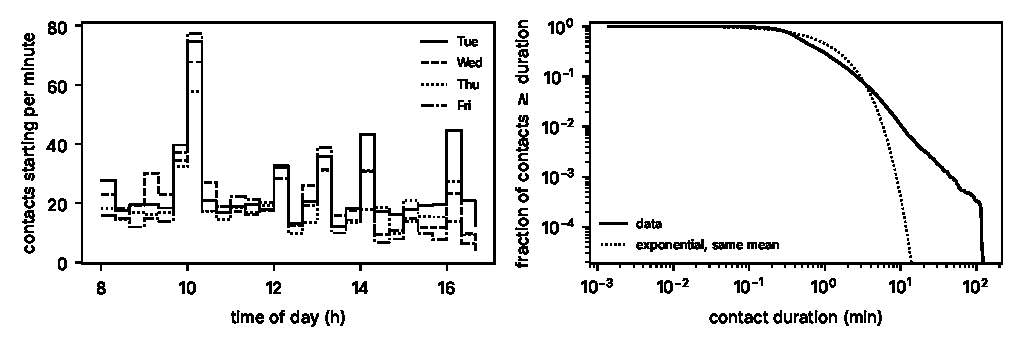
\includegraphics[width=\columnwidth]{generated/fig-data}
\caption{Left: contacts starting per minute over the school day, for the four full days.
The peaks at the start of each hour and at the morning break reflect the timetable.
Right: distribution of contact durations, compared with an exponential distribution of the same mean.}
\label{fig:data}
\end{figure}

The timetable is visible in the data as peaks of contact formation at the start of each hour and during the morning break (Fig.~\ref{fig:data}, left).
It is an exogenous driver, which we include in all models as forced events: at the start of each hour, all students are linked to a hub entity for that hour, during the first 20 minutes of each hour to a hub entity for the change of rooms, and from 10:00 to 10:20 to a hub entity for the morning break.
Rates depend on these links through the numbers of links of each student to the hub entities, and the likelihood is conditional on the forced events.
Pairs that met on an earlier day are linked by a relationship that is also set by forced events at the start of each day.
We use Monday to Wednesday (\EventsTrain\ events) for estimation and Thursday and Friday (\EventsTest\ events) for evaluation.
